\section{Cr�er un compte}

Lorsque l'administrateur souhaite ajouter de nouveaux enseignants, il
se dirige vers la page de cr�ation du compte � l'aide des liens qu'il
dispose dans la zone de liens.\\
Les champs {\it Nom} et {\it Pr�nom} sont des champs obligatoires car
ils sont n�cesssaires � la cr�ation automatique des logins et mots de
passe, ce qui retire � l'administrateur une lourde tache.  
\begin{flushleft}
\scalebox{0.5}{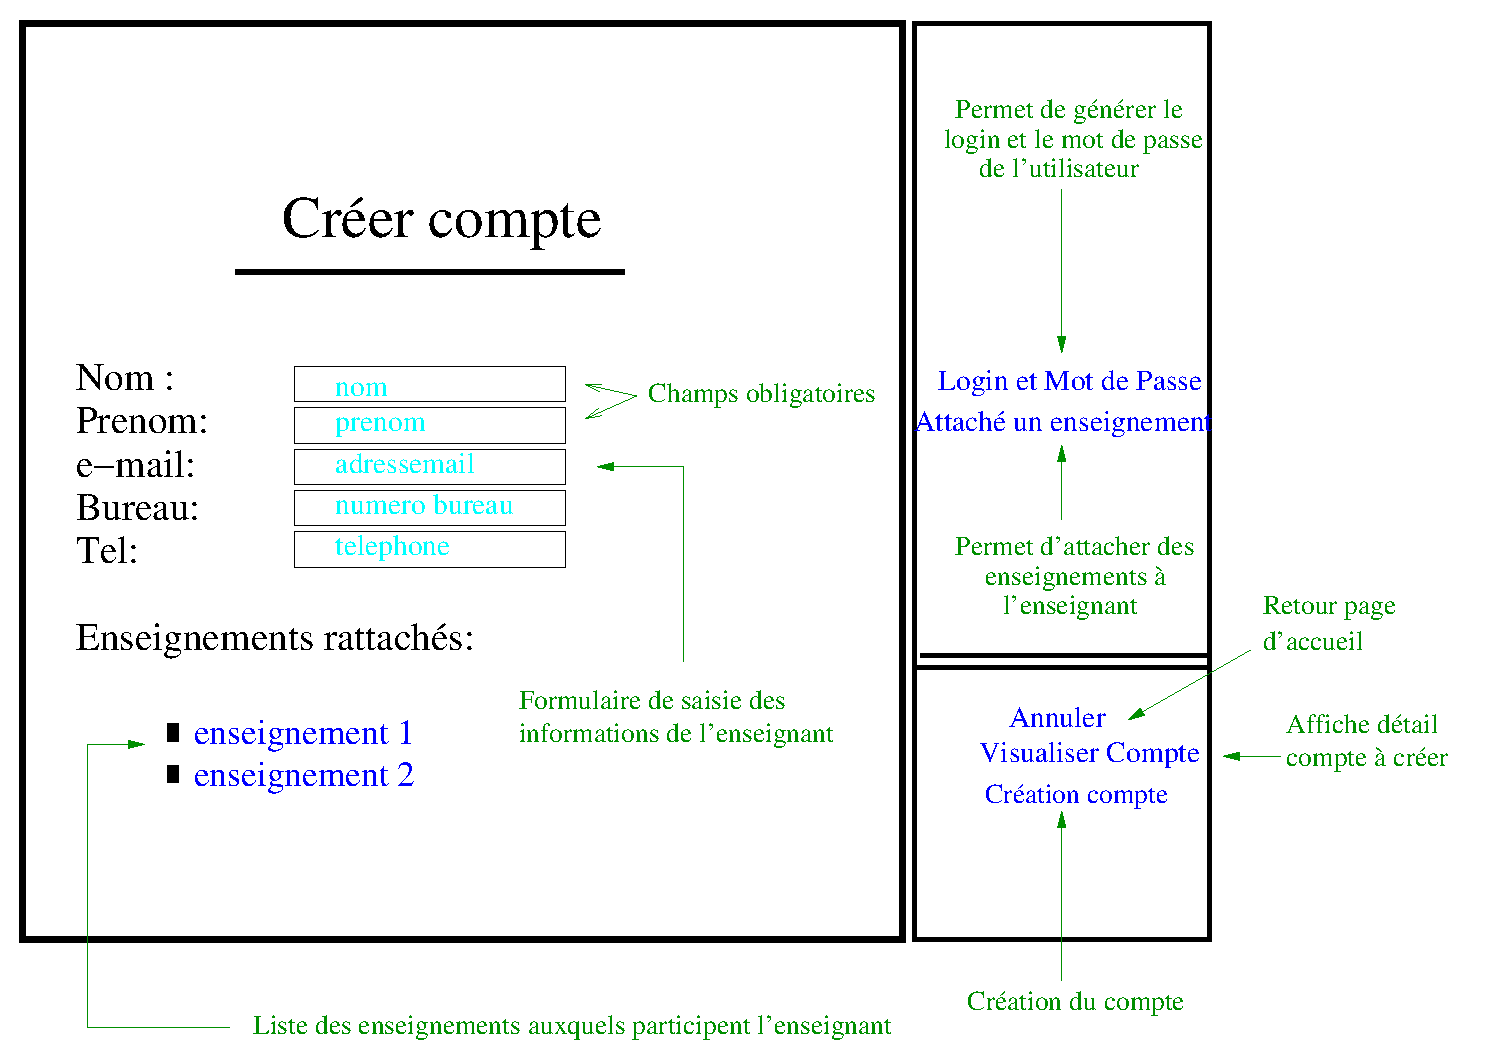
\includegraphics{../eps/compteCreer.eps}}\\
{\it Fen�tre de cr�ation du compte}
\end{flushleft}

L'administrateur a la possiblit� de valider � la cr�ation du compte
mais �galement d'avoir un aper�u du compte.
\begin{flushleft}
\scalebox{0.5}{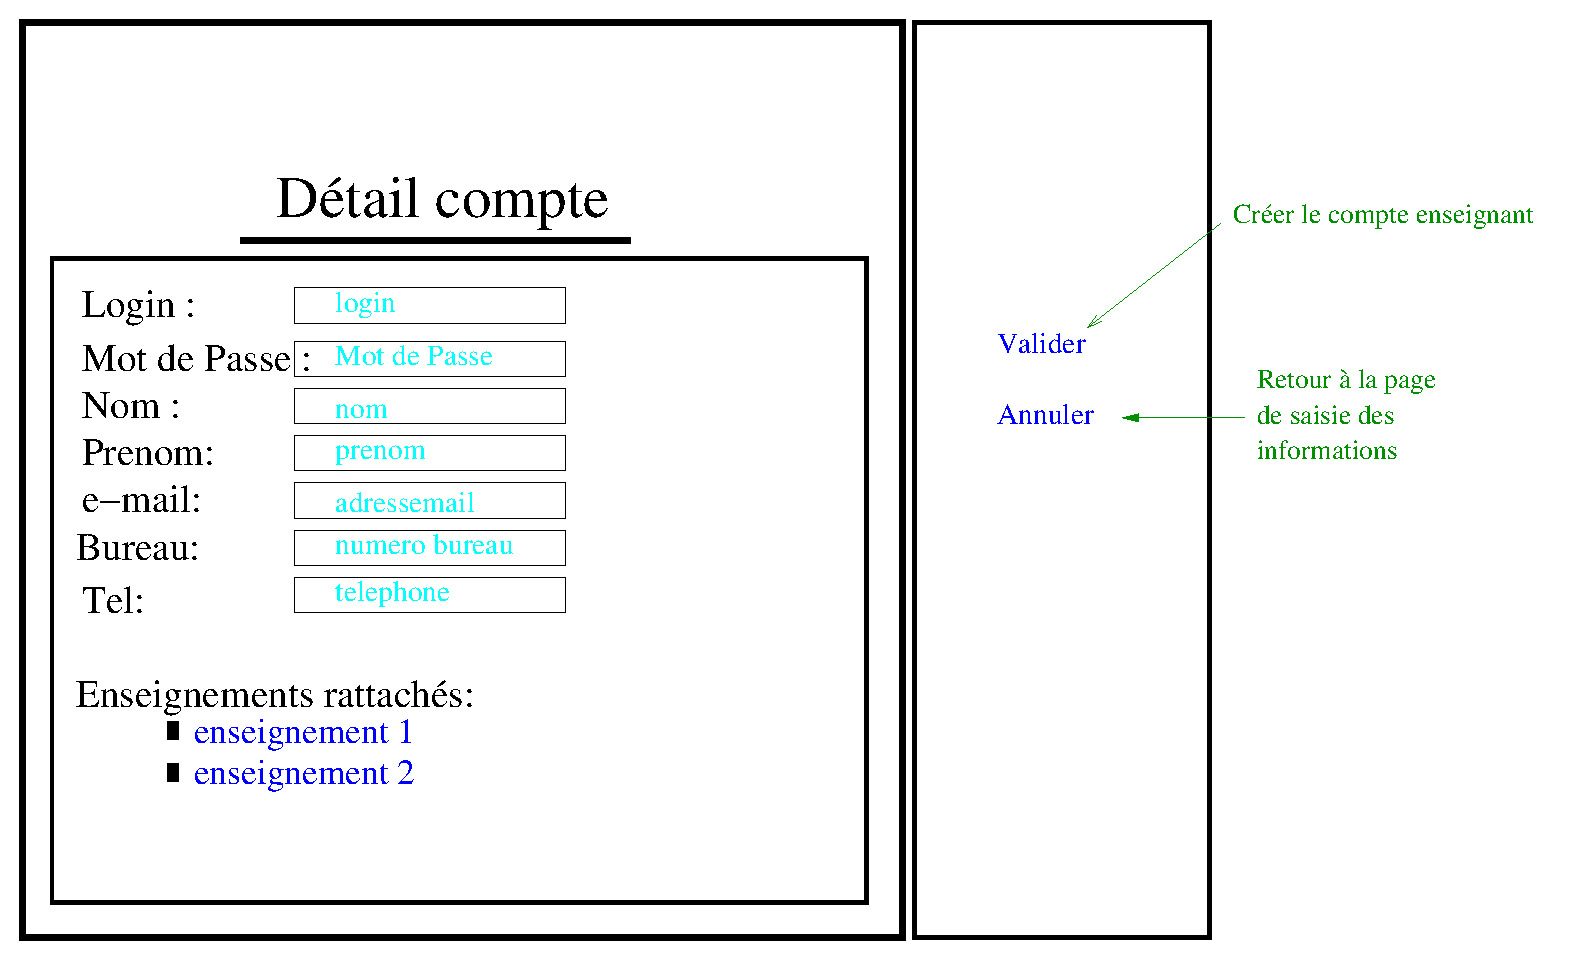
\includegraphics{../eps/compteDemandeConf.eps}}\\
{\it Visualisation du compte avant validation}
\end{flushleft}



